\chapter{Thesis Overview: Astrophysics \& Techniques}
\minitoc
%\pg
%This section aims to provide a general overview of our scientific aims \& chosen strategy. [describe more]

\section{Astrophysical Interest}

\pg
Radio astronomy is a young but extremely dynamic field with a large range of science cases. From the study of the epoch of reionisation, which involves looking for polarised, redshifted 21cm line emission to study the emergence of the first luminous sources\footnote{See \url{https://www.haystack.mit.edu/ast/science/epoch/} for more information - the ultimate goal of this topic is to  learn more about the process of structure formation in the universe: what exactly are the evolutionary links between the very smooth matter distribution revealed by CMB studies and the highly structured universe of galaxies and clusters thereof which we know today?}, to that of variable radio sources such as pulsars and (theoretically) exoplanets, going through the study of ultra-high-energy cosmic rays, solar science, space weather science, the study of cosmic magnetism, and the creation of deep extragalactic surveys, radio-astronomy opens up an extremely fertile window into our Universe. 

\pg
In \cref{fig.meerkat.galcentre}, for example, much structure is immediately visible: supernova remnants in the galactic plane (the ``bubbles"), gas following galactic magnetic field lines (the filamentary structure), and emission from diffuse gas structure around the core of the Milky Way. Other sources are also visible, however: some unresolved sources, and very many AGN sources. This is one particularly striking example of what radio telescopes allow us to see of astrophysical sources, but is only one among many.
\begin{figure}[!h]
	\centering
	\includegraphics[width=\textwidth]{images/{MeerKAT-Galactic-Centre-Low-Res}.jpg}
	\caption{\label{fig.meerkat.galcentre} MeerKAT image of the galactic centre, made by SARAO. This is a low-resolution version of the true image.}
\end{figure}


 
\pg
The work presented here falls under the auspices of the deep extragalactic surveys science project. The underlying scientific motivation behind this Key Science Project or KSP is the study of, among other things, radio-active galactic nuclei, or radio AGNs. A radio AGN is a type of radio galaxy whose emission is dominated by its nucleus. This nucleus emission is non-thermal, and assumed to be emitted from both collimated jets springing from the accretion of matter onto a galaxy's supermassive black hole and from a hot accretion disk surrounding said black hole. AGNs are then commonly split into different types, based on spectral line behaviour \citepads[as in]{1943ApJ....97...28S} or morphological characteristics \citepads[as in]{1974MNRAS.167P..31F}. 

\pg
So-called unified AGN models, which aim to explain the underlying physical object which is assumed to lie behind all observed examples of AGN, were developed to explain the diversity in observed AGN types \citepads[e.g.]{1985ApJ...297..621A,2008A&A...490..893T,2015ARA&A..53..365N,2017MNRAS.469.1883M}. These models would include a central engine, usually a supermassive black hole with hot accretion \citepads[innermost accretion regions estimated to be around $10^7$K by]{1972A&A....21....1P}, emitting thermally; an optically thick disk torus, typically of size 10 to 100pc, blocking light emitted from the central engine along the equatorial plane, and the cavity inside which would be the region from which broad emission lines would emit; and finally, ionisation cones in the direction of the poles, where the emission from the central engine would collimate into large-scale jets (which would also, at the scale of a few tens of parsecs, create the region of narrow spectral line emission).


\pg
The interaction between AGN jets and the surrounding intergalactic medium can result in structure such as that shown in \cref{fig.agn} below: the bright nucleus of a radio galaxy in the centre of two extremely radio-bright jets, with lots of diffuse emission from their lobes. These lobes show where the accretion-accelerated particles begin to slow down - and therefore emit - due to contact with the intergalactic medium. Hence, their sometimes peculiar shape: this medium can be complex and inhomogeneous (if the radio galaxies lie in a cluster, for example) which can lead to the sort of jet structure shown in this image.
\begin{figure}[!h]
\centering
\includegraphics[width=0.6\textwidth]{images/{3C31_radio_optical_montage_Alan_Bridle}.png}
\caption{\label{fig.agn} Radio optical montage of 3C31, by Alan Bridle: \url{https://www.cv.nrao.edu/~abridle/3c31xopt.htm}.}
\end{figure}

\pg
Of course, not all galaxies have active nuclei, and those which do also have other forms of radio emission: for example, free-free radiation from the interstellar medium, ionised by light from newborn stars, will often contribute to radio-galactic flux. Some galaxies with active nuclei do not have strong jet emission: these are called radio-quiet AGNs. We can thus identify two components to a radio AGN: the host galaxy and its jets. Peak star formation is thought to have occurred around $z\sim2$, and so the study of AGN activity around this period is of strong scientific interest. Could the jets from active AGNs have contributed to the decline in star formation? Are there large populations of older AGNs, and if so, how old? These are the astrophysical questions which motivate the study of AGN sources \citepads{2007NewAR..51..168B,2018arXiv180501544X,2018ApJ...853...24U}, which is the driving scientific concern which motivates the present doctorate.
%
%\pg
%Both of these components tell us different things about the galaxy and its surrounding medium. If the host galaxy can be resolved out from the jets, for example, it becomes possible to study the star formation history of that galaxy by comparing the radio flux at different frequencies to the galaxy's brightness in other bands (X, IR, optical etc). Radio waves are not subject to extinction in the way that infrared or optical emission can be: this fact needs to be taken into account when performing this sort of analysis.
%
%\pg




\clearpage

\section{The Low-$\nu$ Sky: Emission Mechanisms}
\pg
This section aims to bring a brief introduction to the emission mechanisms which dominate at low frequencies, and thus determine the physics accessible to extragalactic astronomers working in this band. Specifically, it will briefly describe
free-free radiation (which is emitted from ionised plasma outflows, and thus a tracer of various physical objects e.g. young stellar objects - cf. \citet{2017ApJ...834..206C} and references therein - and starburst regions - cf. \citet{2015A&A...574A.114V}) and synchrotron radiation, which is a tracer of more violent and energetic processes (and thus associated with supernova remnants, AGN, or radio halos - cf. \citet{2010A&A...509A..68C}).

\pg
Of course, each individual galaxy will have differing contributions from different mechanisms - in practice, when studying galactic populations, the overall flux at a given frequency will simply be summed up for each galaxy and become one point in a Spectral Energy Distribution, or SED. However, when studying individual objects, it can be critical to understand which emission mechanism dominates at what frequencies. For example, the radio and far-infrared spectrum for nearby M82 are shown in Fig. \ref{plot.m82.spectrum}\footnote{Figure and work taken from the NRAO website. For further information, \href{https://www.cv.nrao.edu/course/astr534/FreeFreeEmission.html}{see here}}: \url{https://www.cv.nrao.edu/course/astr534/FreeFreeEmission.html}.
\begin{figure*}[!h]
\centering
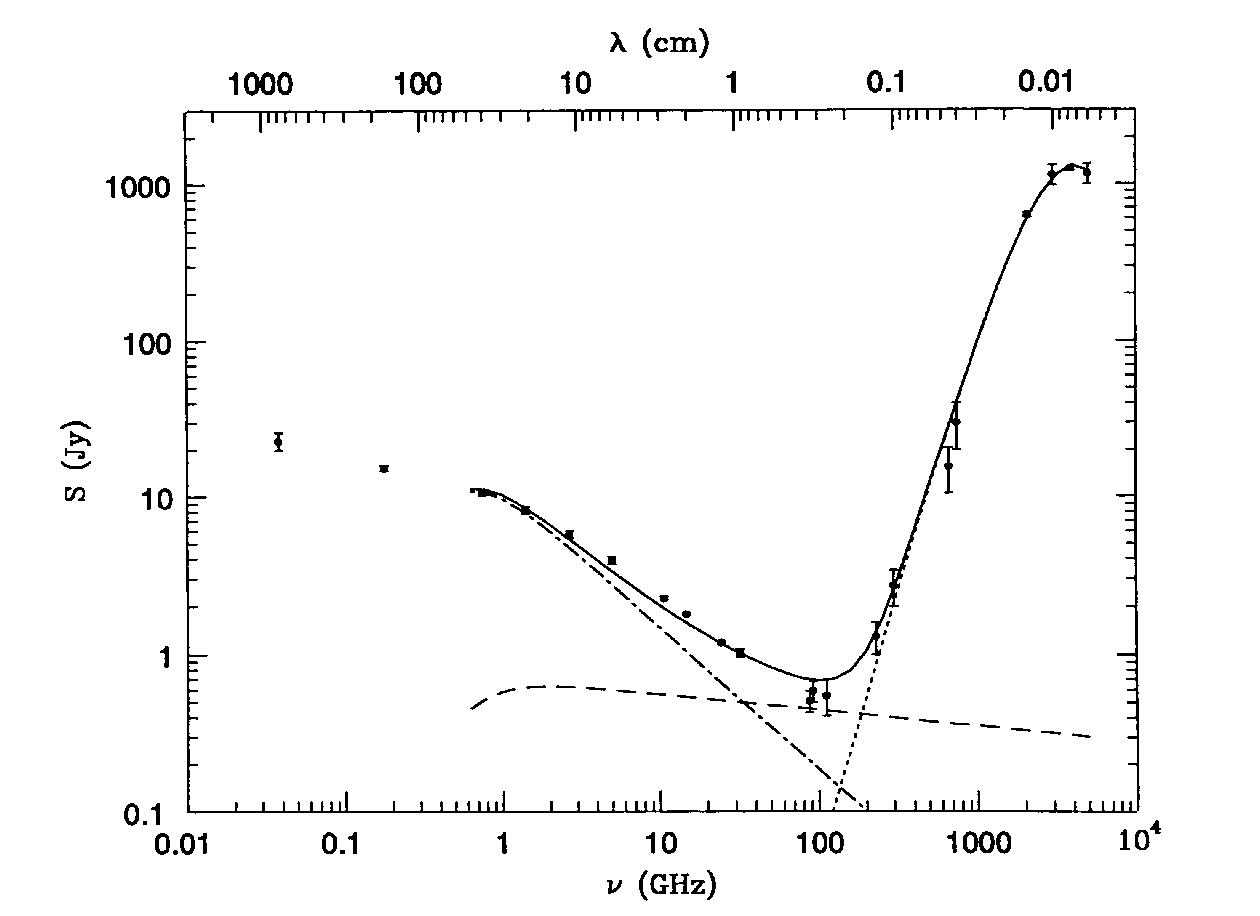
\includegraphics[width=\textwidth]{images/M82Spectrum.png}
\caption{\label{plot.m82.spectrum} Radio and far-infrared spectrum for galaxy M82, as estimated \href{https://www.cv.nrao.edu/course/astr534/FreeFreeEmission.html}{by the NRAO online course} (\url{https://www.cv.nrao.edu/course/astr534/FreeFreeEmission.html}). The flat curve corresponds to free-free emission, while synchrotron radiation (negative slope) and thermal dust emission (postive slope) dominate at low and high frequencies respectively.}
\end{figure*}


\subsection{Synchrotron Radiation}

\pg
Synchrotron radiation is the dominant mode of emission for extragalactic sources at low wavelengths. As such, it will be covered in greater detail than the other mechanisms above, which are important in other bands (and therefore relevant for multi-spectral analysis) but much less relevant to LOFAR observations. This section draws heavily from Garret Cotter's \href{http://www-astro.physics.ox.ac.uk/~garret/teaching/}{high-energy astrophysics lectures}\footnote{\url{http://www-astro.physics.ox.ac.uk/~garret/teaching/}}, as well as Alan Loh's \href{http://theses.md.univ-paris-diderot.fr/LOH_Alan_2_va_20160930.pdf}{doctoral thesis} \citepads{alan} and \href{https://www.cv.nrao.edu/course/astr534/SelfAbsorption.html}{the NRAO online course}\footnote{\url{https://www.cv.nrao.edu/course/astr534/SelfAbsorption.html}}.

\pg
Synchrotron radiation (or ``magnetobremsstrahlung") occurs when the trajectory of a relativistic charged particle is guided by a magnetic field. As the German name suggests, it is the magnetic equivalent of free-free radiation. It is the tracer of very energetic processes, such as the interaction between AGN jets and the intergalactic medium. In the low-energy regime, it is also known as cyclotron radiation, after the device in which it was first measured in a laboratory. %, and in non-relativistic regimes, it is known as gyro radiation. 

\pg
The synchrotron power spectrum of a population of electrons with exactly the same energy is a function of its Lorentz factor and its emission angle\footnote{The emission angle is the angle between the electron's total velocity (including z-axis) and its radial velocity.} \citepads{1994hea2.book.....L}. The typical radiation spectrum for a single electron is shown in \cref{fig.synchrotron.1electrion} as a function of the critical frequency, which is itself a function of the emission angle $\theta$, the Lorentz factor $\gamma$ and the magnetic field strength $B$: $\nu_c=3/2\frac{\gamma^2 e B}{2\pi m_e c}\sin(\theta)$. $e$ and $m_e$ are the electron charge and mass, respectively.
%$\nu_c=3/2\frac{\gamma^2 e B}{2\pi m_e c}\sin(\theta)$.
\begin{figure}[!h]
\centering
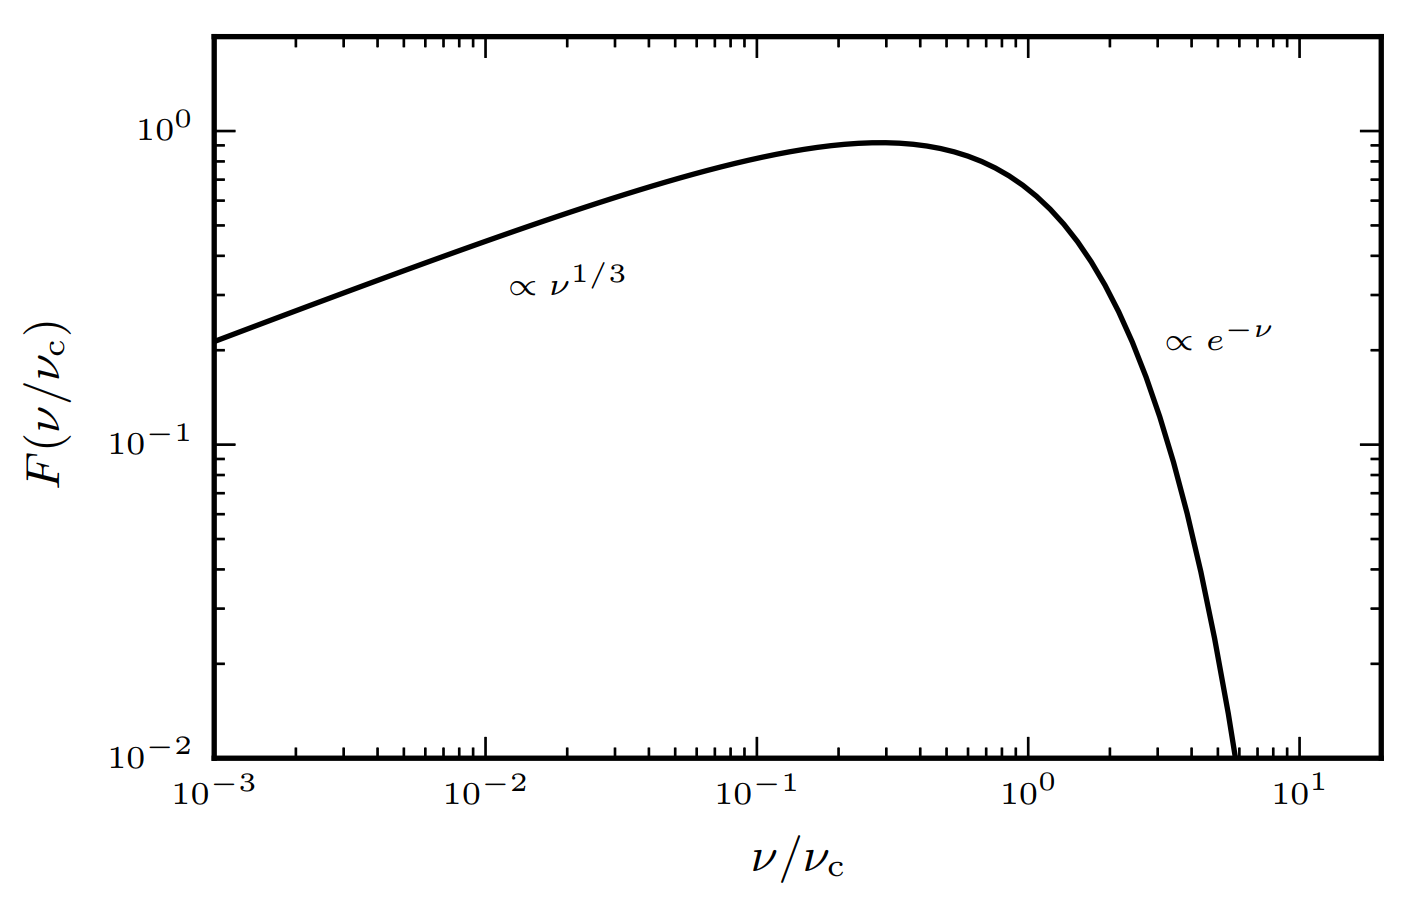
\includegraphics[width=0.9\textwidth]{images/Synchrotron-single-electron.png}
\caption{\label{fig.synchrotron.1electrion} Characteristic spectrum of synchrotron emission for a population of single-energy electrons. Arbitrary unit scale. Source: NRAO online course: \url{https://www.cv.nrao.edu/~sransom/web/Ch5.html}}
\end{figure}

\pg
Of course, in reality, we know that electron populations in astrophysical sources do not all share exactly the same energy when emitting. The effect of the electron energy distribution must therefore be taken into account. Because the population in question is energised through non-thermal processes, its energy distribution is not Maxwellian, and is generally written as a power law: $S(E) \propto E^\alpha \rightarrow S_\nu \propto \nu^{-\alpha}$, where $\alpha$ is the object's spectral index. Note that the index of the energy distribution (which relates the number of electrons at a given energy) is different from the synchrotron index, with the two related by the following equation: $\alpha=-(\gamma-1)/2$.
The question now becomes: what $\alpha$ is appropriate for what kind of object? Does every source have the same $\alpha$ at all frequencies? Do all synchrotron sources have the same spectral index at a given frequency, and if not, what does this tell us?

\pg
To answer these questions, we must recall that so far, we have assumed that every photon emitted through synchrotron radiation reaches us. This is not necessarily the case in practice: it is possible for a given photon to be scattered (i.e. absorbed \& re-emitted) by surrounding high-energy electrons. The likelihood of this occurring at a given frequency is a function of the absorption cross-section, and is a complex quantity to calculate (see \citetads{1994hea2.book.....L}  pp258-260). Suffice to say that at longer wavelengths (lower frequencies) absorption is more effective, and at shorter wavelengths (higher frequencies) the underlying electron energy power-law  distribution begins to dominate. An example is shown in \cref{fig.synchrotron}, taken from \citetads{2007A&A...471.1105T}.

\begin{figure}[!h]
\centering
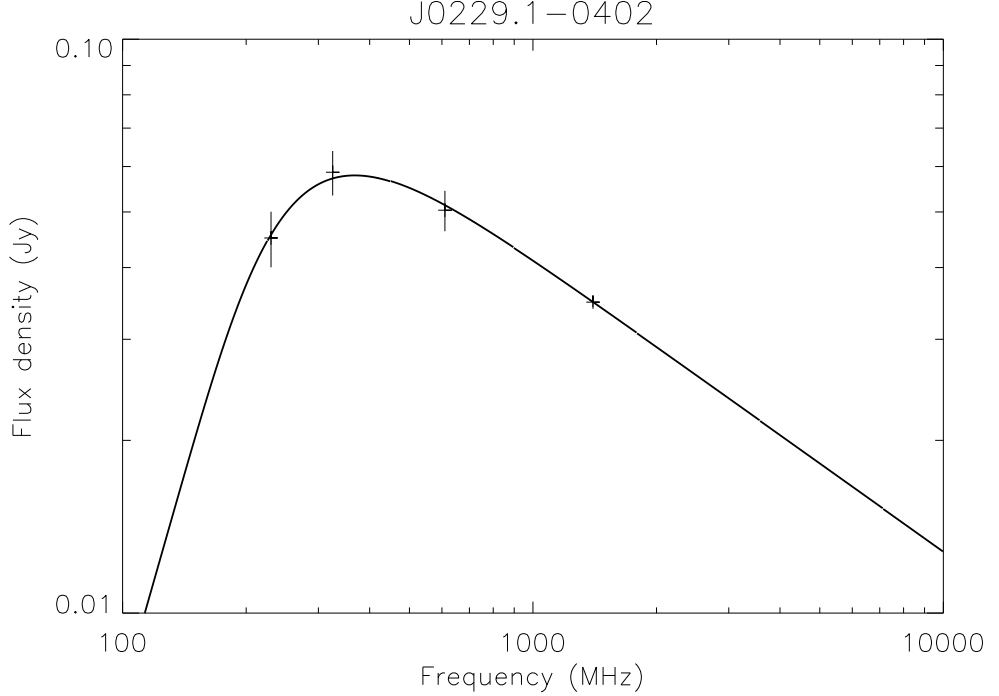
\includegraphics[width=0.8\textwidth]{images/synchrotron-spectrum.png}
\caption{\label{fig.synchrotron} Power spectrum for J0229.1-0402. Source: \citetads{2007A&A...471.1105T}.}
\end{figure}

\pg
In the optically-thick regime, we know that the most efficient radiation mechanism is simple black-body radiation, and so the power spectrum at a given frequency can be defined in terms of an ``electron temperature". In the Rayleigh-Jeans approxmation (valid as we are explicitly in the low-frequency regime), this gives $S_\nu \propto \nu^{5/2}$, or $\alpha=5/2$. 
In the optically-thin regime, meanwhile, we recover a mixture of the underlying power-law distribution ($S_\nu \propto \nu^{-\alpha}$) and black-body radiation (which has a frequency-dependent $\alpha$). Empirically, we generally observe $\alpha \sim 0.7$.


\subsection{Free-Free Radiation}
\pg
Free-free or ``bremsstrahlung" (``braking") radiation occurs when the trajectory of a charged particle is deflected by an electric field. This non-thermal emission mechanism is the dominant mechanism in HII regions (which contain ionised hydrogen), where star formation has previously taken place. It is called free-free emission because it is produced by free electrons deviating off ionised hydrogen (i.e. protons) without being captured. When the underlying electron distribution is Maxwellian, it is referred to as thermal Bremsstrahlung.

\pg
This emission's spectrum is heavily dependent on a number of factors: including frequency, temperature, and critically, free-free opacity $\tau_\nu$, itself a function of electron density. It is characterised by a knee in its spectrum, occurring where $\tau_\nu\sim 1$. This knee delineates two regions with different spectral indices; $\alpha \sim -0.1$ at higher frequencies, and $\alpha \leq 2$ at lower frequencies. This gives a characteristic shape, shown in Fig. \ref{plot.freefree.spectrum}.
\begin{figure*}[!h]
\centering
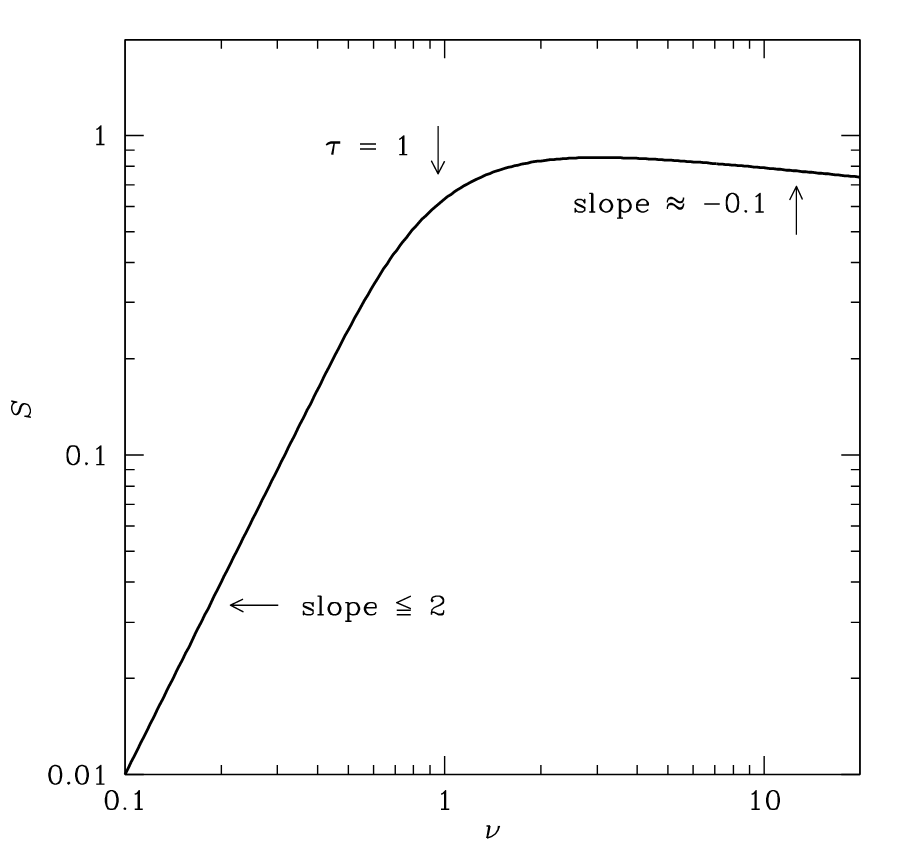
\includegraphics[width=0.7\textwidth]{images/freefree.png}
\caption{\label{plot.freefree.spectrum} Characteristic spectrum of free-free radiation. Arbitrary unit scale. Source: NRAO online course: \url{https://www.cv.nrao.edu/course/astr534/FreeFreeEmission.html}.}
\end{figure*}

\pg
As we can see, this spectrum falls off sharply with decreasing frequency. As such, while it is expected to dominate over thermal emission in the absence of synchrotron radiation, it is synchrotron emission that is expected to dominate overall - if present - at the low frequencies of our observations, which are done with LOFAR. Free-free emission acts as a tracer for star formation and other "gentler" physical processes detected at low radio frequencies.



\clearpage
\section{LOFAR: The LOw-Frequency Array}

\pg
Our observations have all been made with the LOw Frequency Array LOFAR \citepads{2013A&A...556A...2V}. In this section, we describe its technical properties and its current state of the art. In particular, the distinction between ``Dutch" LOFAR and ``international" LOFAR - and the technical problems associated with each - will be made explicit in this section.

\pg
LOFAR is a SKA pathfinder instrument, which means that it serves not only as a cutting-edge instrument in its own right, but does so with the explicit aim of serving as testing grounds for technologies \& techniques which could be usefully implemented in the SKA. It is in this context, for example, that trailblazers such as NenuFAR \citepads{2012sf2a.conf..687Z}, a low-frequency extension of LOFAR, are tested. LOFAR is an interferometric array, with each of its elements made up of antennas combined into a phased array, themselves forming an interferometer. It thus consists of antennas which are combined to form stations, which are themselves distributed throughout the Netherlands and Europe.
\begin{figure}[h!] 
  \begin{minipage}[c]{0.45\linewidth}
    \centering
    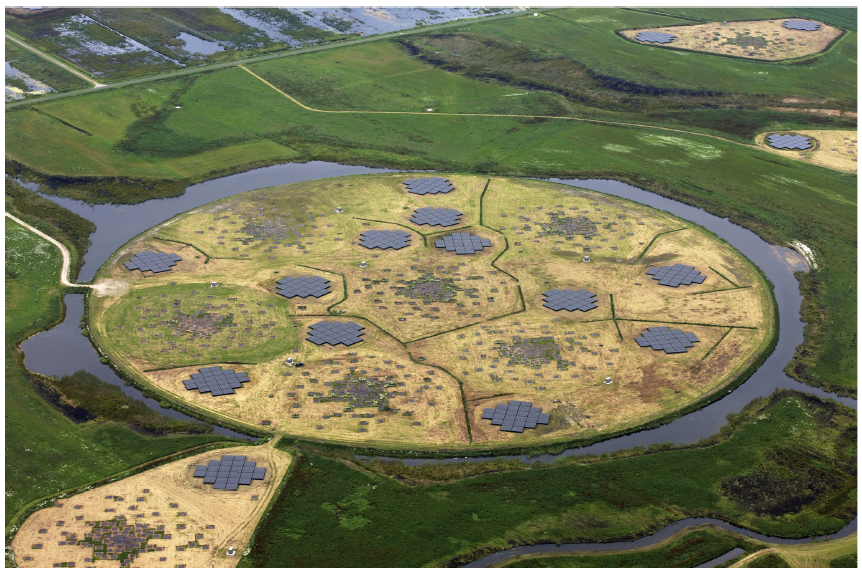
\includegraphics[width=\linewidth]{images/superterp.png}
	\subcaption{\label{fig.lofar.superterp} LOFAR core, known as the Superterp.}
%    \vspace{4ex}
  \end{minipage}
  \hfill
  \begin{minipage}[c]{0.45\linewidth}
    \centering
    \includegraphics[width=.5\linewidth]{images/{lofar-core-map_grey.jpg}}
    \subcaption{\label{fig.lofar.core} Distribution of the so-called LOFAR "core" stations, which include the Superterp.}
%    \vspace{4ex}
  \end{minipage} 
  \begin{minipage}[c]{0.45\linewidth}
    \centering
    \includegraphics[width=\linewidth]{images/{Distribution_Remote_Stations}} 
    \subcaption{\label{fig.lofar.remote} LOFAR with both "core" and "remote" stations.}
%    \vspace{4ex}
  \end{minipage}
  \begin{minipage}[c]{0.45\linewidth}
    \centering
    \includegraphics[width=.9\linewidth]{images/{Distribution_International_Stations}} 
    \subcaption{\label{fig.lofar.international} International LOFAR. Newer stations (one in Ireland, three in Poland) are not shown here.}
%    \vspace{4ex}
  \end{minipage} 
\caption{\label{fig.lofar.distribution} Geographic location and distribution of LOFAR stations, explicitly showing what is meant by Superterp, core, remote and international stations. All images from \href{https://www.astron.nl/radio-observatory/astronomers/users/technical-information/lofar-array-configuration/lofar-array-conf}{the official ASTRON website}: \url{https://www.astron.nl/radio-observatory/astronomers/users/technical-information/lofar-array-configuration/lofar-array-conf}}
\end{figure}


\pg
There are two bands to LOFAR, which are known as LOFAR-HBA (High-Band Antennas) and LOFAR LBA (Low-Band Antennas). \cref{fig.lofar.superterp,fig.fr606.layout} show the layout of the 6 innermost core stations and the French international LOFAR station, respectively.
\begin{figure}[h!]
\includegraphics[width=0.5\textwidth]{images/{LOFAR_NenuFAR.jpg}}
\caption{\label{fig.fr606.layout} Layout of FR606, the French LOFAR station at Nancay. At bottom left are the HBA tiles, bottom right the LBA dipoles, and at the top are some of the NenuFAR tiles.}
\end{figure}



\pg
We see the presence, in both cases, of two very different antenna types. One of these antenna types is not a single antenna, but rather a phased array: 16 antenna dipoles distributed in a $4 \times 4$ array. International LOFAR stations include 96 such tiles, distributed in a ``filled-disk" pattern, where the disk fill ratio is determined by the size of the tile. Dutch ``remote" stations have 48 such tiles spread into 2 disks (HBA\textunderscore INNER and HBA\textunderscore OUTER), while ``core" station HBA tiles are split into two 24-tile crosses. This pattern is shown in \cref{fig.hba.tile}. The antennas from each tile are combined into a phased array with a single ``tile beam", and all tile beams are themselves combined as a phased array into a station beam\footnote{Reference: \href{https://www.astron.nl/radio-observatory/astronomers/technical-information/antennae/antennae-description}{ASTRON technical description}: \url{https://www.astron.nl/radio-observatory/astronomers/technical-information/antennae/antennae-description}}.% This station beam is then pointed digitally.
\begin{figure}[h!]
\includegraphics[width=0.45\textwidth]{images/{Schematic-diagram-of-a-24-tile-LOFAR-HBA-station-A-tile-is-made-of-16-dual-polarization.png}}
\caption{\label{fig.hba.tile} Layout of a single HBA tile. Source: \href{https://www.researchgate.net/profile/Sarod_Yatawatta/publication/281316394/figure/fig1/AS:614002589720576@1523401033149/Schematic-diagram-of-a-24-tile-LOFAR-HBA-station-A-tile-is-made-of-16-dual-polarization.png}{Sarod Yatawatta researchgate profile}}
\end{figure}



\pg
LBA antennas, use a very simple - and cost-effective - design. A typical LBA antenna is shown in \cref{fig.lba.ant}. 96 such antennas are spread in a semi-random pattern in each LOFAR station\footnote{Reference: \href{http://www.lofar.org/about-lofar/system/lofar-numbers/lofar-numbers}{LOFAR.org website}: \url{http://www.lofar.org/about-lofar/system/lofar-numbers/lofar-numbers}}. In Dutch stations, 48 of these are used at all times. They are combined as a single phased array.
\begin{figure}[h!]
\includegraphics[width=0.45\textwidth]{images/{lba.png}}
\caption{\label{fig.lba.ant} Picture of a single LBA antenna. Source: \href{https://i2.wp.com/lofar.ie/wp-content/uploads/2017/04/lba.png?resize=1500\%2C1000}{LOFAR technology website.}}
\end{figure}
\pg
LOFAR-HBA is sensitive to higher frequencies, from 120 MHz to 240 MHz\footnote{Reference: \href{http://www.lofar.org/about-lofar/system/lofar-numbers/lofar-numbers}{LOFAR.org website}: \url{http://www.lofar.org/about-lofar/system/lofar-numbers/lofar-numbers}}. It has a smaller field of view than LOFAR-LBA, but a better angular resolution. 
\pg
The dipole design frees observers from the need to physically point antennas at all: the final station pointing is achieved by digitally introducing delays in the recorded phase before averaging the data. In this sense, the pointing is achieved in a similar way as individual HBA tile pointing, albeit . The LBA antennas are receptive to signals emitted in the 30-80 MHz frequency range.

\pg
At the time of writing, use of the LBA data is still relatively new, as its calibration is a very tricky problem. For similar reasons, international LOFAR (i.e. the full LOFAR array) has not been used, at the time of writing, to create wide-field survey images. A large part of the work described in this manuscript consists of reaching a point where full use can be made of international LOFAR, in a streamlined and repeatable way. 



\clearpage
\section{This Thesis}

\pg
The work done in this thesis can be summarised as the development of a new algorithm for mitigating calibration artefacts in radio-interferometric images, and its application to a peculiar famous extragalactic field. Because our data volumes put radio interferometry in the domain of ``Big Data" (there are $\sim$245TB of LOFAR data centred on the Extended Groth Strip, for example), there is a very real need for fast, reliable methods with which to improve interferometric images. This algorithm follows from an improved understanding of the noise properties of interferometric images, and can be understood as a way to better constrain the flux distribution in images by minimising the presence of artefacts. This, in turn, helps self-calibration convergence by improving the image resulting from each imaging step of the self-calibration process. 

\pg
We then outline the application of this work, along with other modern tools, to the creation of a large, deep and high-resolution image of a rich patch of sky. While this approach is potentially extremely rewarding in terms of the science one can do with its resulting maps, it is also uniquely complicated. There exist many LOFAR HBA ($\sim$120-240 MHz) sky surveys \citepads[cf.]{2016MNRAS.460.2385W,2017A&A...598A.104S}, but they do not yet make use of international LOFAR, and are thus limited in resolution ($\sim 5''$). And while there are surveys made at LOFAR frequencies ($\sim$150MHz) with other instruments \citepads[e.g.]{2017A&A...598A..78I}, they do not match the resolution attainable with international LOFAR. The aim of our image is then to show that the international LOFAR stations can be used to create a radio image that matches HST/ACS resolution - which would allow for significant cross-matching and source analysis, since there is HST data available for the field being imaged, the Extended Groth Strip (EGS). This would not be a true survey, but more of a proof of concept: the application of new tools and the development of an appropriate strategy to image a large patch of the sky with the full LOFAR array. This image would have better resolution than FIRST \citepads[see][and references therein]{2015ApJ...801...26H}, which has a $4''$ resolution, relatively low sensitivity, and no short baselines (thereby missing diffuse emission and extended structure) at $\sim$1.4 GHz, while still being sensitive to diffuse emission due to the use of the LOFAR core stations. 
%Finally, there will of course be the SKA1-MID survey once the SKA is operational; this survey is expected to provide excellent resolution, sensitivity, and good $uv$-coverage, making it sensitive to diffuse emission as well as point sources.

\pg
Making this image is possible only because LOFAR observations of the Extended Groth Strip includes an extremely bright source, 3C295, in their field of view. This is both a blessing and a curse: unless this source is properly modeled and subtracted, it will pollute images of the EGS. However, because it is so bright, it can serve as a good calibrator source for the LOFAR international stations - if a good enough model of 3C295 can be made and used to calibrate these stations, then high-resolution images of the EGS becomes attainable. This would give access to a large population of radio AGNs at high resolution, observed at a large range of frequencies, and many of which lie at redshifts near the peak of star formation; this improvement of our low-frequency understanding of these objects could, in turn, lead to an improved understanding of these objects more generally.

\pg
To really be able to perform wide-field images using the full LOFAR array, we cannot rely on the happy circumstances we find ourselves in for our applications project: a much more thorough and reliable approach is necessary. The work of the LOFAR long-baseline team \citepads[e.g.]{2016A&A...595A..86J} shows that kind of approach: in our project, we test specific strategies and approaches which are complimentary to their work, but cannot be applied more generally without their results.

%\pg
%In this context, a sky survey made using international LOFAR would be competitive until the SKA-MID survey (and considering it maps the Northern sky rather than the Southern sky, would arguably remain competitive even then). It would also allow LOFAR to fulfill the role of pathfinder in a very literal way, by providing datasets on which algorithms and imaging strategies could be tested before handling SKA data volumes in real-time.
%
%\pg
%Making a high-resolution full-sky survey using international LOFAR is thus arguably useful in and of itself in terms of interferometric techniques \& instrumentation. What then of its science value? The two most obvious advantages of a good large-sky survey are that they are complete (i.e. they are an accurate sample of the underlying source distribution, up to the survey's limiting flux)  while still giving information on rare outlier objects which may happen to lie in the field. This gives us access to a wealth of statistics from which to derive more robust estimations of population distributions. %Furthermore, depending on the quality of a given survey, it might even be able to provide such statistics simultaneously for various different fields of scientific interest.
%
%\pg
%Of course, LOFAR is already providing such catalogues - LOTSS \citepads[see][and references therein]{2017A&A...598A.104S}  is only the first of many to come. But these catalogues do not make use of the LOFAR international stations, and thus do not make full use of LOFAR's resolution ($5''$ resolution vs. $0.5''$).  This is so due to the technical challenges introduced by the use of international stations, which are due to decorrelation and an already limited signal-to-noise on those very short spatial frequencies.
%
%\pg
%What would they add to a LOFAR catalogue? A high-resolution sky survey has all the advantages listed above with more besides. For AGN science, for example, the higher resolution gives information on smaller scales, which is very relevant to study the turbulent processes in the lobes and the nearby intergalactic medium. This can give better insight into AGN feedback, for example \citepads[e.g.]{2007NewAR..51..168B,2016A&A...593A.118Q}. We also know that there exist small AGNs: size therefore matters, and resolving these small AGNs (which tend to lie at larger redshifts, hence their smaller angular size) can give extremely salient information on AGN population distributions as a function of the age of the universe. Indeed, for AGN science, the LOFAR international baselines can be the difference between having absolutely no information on size distribution (no resolved AGN) and knowing everything about the AGN size distribution within a given extragalactic field. Finally, resolving sources is very relevant to spectral studies of AGN populations: we know very little about the physics of AGNs at low frequencies. Information on large populations of resolved sources (allowing us to separate compact structure from extended emission) is a prerequisite to begin the statistical work needed to understand these low-frequency AGN physics. As such, the international baselines can bridge a critical gap in the data available to peers studying AGN science.
%
%\pg
%AGN science is far from the only field which could benefit from the sub-arcsecond resolution that international LOFAR could provide. High-resolution imaging can be of tremendous interest to the study of star-forming galaxies: it could give insight into cosmic ray structure and access to spectral information. This is relevant because the entire star-forming history of galaxies is encoded in radio emission, but can only be accessed with sufficient spectral information and spatial resolution. A high-resolution survey, in particular, allows comparisons between optical and radio emission for known star-forming galaxies on a truly industrial scale, which would allow for the mapping of free-free absorption, supernova remnants, HII regions, etc...onto optical maps, and this for sources going up to high redshifts.
%
%\pg
%Of course, this does not run the full range of science cases which would benefit from high-resolution maps of large parts of the radio sky. Colleagues studying gravitational lensing would benefit greatly from large samples of lensed galaxies. Resolved extragalactic recombination lines (for bright objects) would doubtlessly interest peers studying galactic evolution. We expect these samples to be a natural byproduct of a large, high-resolution map of the radio sky: if they do not appear, that could indeed be a very interesting scientific result in and of itself.
%
%\pg
%More generally, high-resolution surveys provide high-resolution images of everyone's favourite objects and sources. It allows for better optical matching and identification, which is particularly relevant e.g. when needing to associate either a low-z or high-z sources to optical counterpart sources (in the case of the Extended Groth Strip, for example, using the international stations means matching the Hubble Space Telescope's resolution). They are thus a strong contribution to multi-wavelength datasets. It also improves the image's sensitivity to compact sources embedded in diffuse emission: if the source is better-resolved, then the emission associated with compact sources is more easily separated from emission emitted by its surroundings. This can be of tremendous help in image interpretation. Finally, actually resolving objects allows us to have better morphological classification for compact objects, which can be extremely useful e.g. when interested in AGN populations vs star-forming galaxy populations.

\subsection{Algorithmic Developments}

\pg
A significant portion of the work done as part of this thesis was on investigating the relationship between calibration gain errors and calibration artefacts in the image-plane. What started as an attempt to properly write a weighting scheme to down-weigh poorly-calibrated visibilities\footnote{i.e. to justify weighting visibilities by a function inversely proportional to the variance of the associated residual visibilities.} eventually became a formal relationship between these quantities, showing both the behaviour of image-plane variance as a function of direction but also of pixel covariance over the full image. This work is shown in much greater detail in \cref{chapter.paper}.

\pg
The key finding of our algorithmic work is a fundamental relationship between the covariance matrices of residual visibilities and the covariance of pixels in the image-plane: the ``Cov-Cov relationship'' between visibility covariance and image-plane covariance. The pixel variance and covariance in the image-plane are determined by a ``noise-PSF'', convolved with every pixel in the sky. This also means that thermal noise in interferometric images is correlated between pixels, and that this correlation is given exactly by the PSF: in the limit of an empty, non-deconvolved sky, we therefore properly model the thermal noise properties of its interferometric images. This noise-PSF is the product of the Fourier transforms of the calibration gain covariance matrix with each cell mapped not from $uv$ space to $lm$ coordinates\footnote{$uv$ space is where interferometric measurement coordinates lie, and $lm$ coordinates are the cardinal sines on which the inverse Fourier transform of the visibilities are mapped.} but rather between their respective covariance spaces - from a new {differential Fourier plane (henceforth ``$\left(\deltu\deltv\right)$''-plane) to the image-plane covariance space $\deltl\deltm$. This image-plane covariance space describes} the variance in each pixel and the covariance between pixels\footnote{{The noise-PSF also relates $\delta w$ to $\delta n$, as shown in our matrix formalism, but we do not explicitly reference this in the text for the sake of brevity, as visibility space is usually referred to as ``the UV-plane'' in literature, rather than ``the UVW-space''. For more information, see \cref{chapter.paper}}}. It describes the expected calibration artefacts and noise level around each source, does not vary as a function of direction, and is convolved with each source in the field to yield the final error map. Because all unwanted (in our case, unphysical) signal can be thought of as noise, we will refer to {the pixel variance map} as the ``noise-map''.

\pg
Based on this theoretical finding, we develop a weighting scheme algorithm with which to improve the noise properties of interferometric images by down-weighting either visibilities with high variance in their calibration residuals, or visibilities which are strongly correlated to others in their calibration residuals. We implement a robust version of the first weighting scheme, which relies on an antenna-based estimate of the visibility variance. 


\subsection{Imaging the Full Primary Beam}


\pg
In this section, we briefly describe previous observations of the Extended Groth Strip (EGS), an extragalactic field with a rich multi-wavelength coverage described in Table \ref{table.EGS.observation}. It has been long observed as part of the All-Wavelength Extended Groth Strip International Survey collaboration (AEGIS, \citetads{2007ApJ...660L...1D}), which later became part of the CANDELS collaboration (\citetads{2011ApJS..197...35G}). The field is centred at $\alpha=14^h17^m,\delta=+52^o 30'$, placing it between the tail of Ursa Major and Draco. Its size is $0.7'\times 0.1'$. It has notably been the subject of very deep Hubble Space Telescope observations, which the international LOFAR could attempt to match. 

\begin{table}[h!]
\begin{tabular}{cccc}
Telescope    & Band    & Resolution  & Area \\\hline
Chandra      & X-ray   & $0.5''-6.0''$ & $17'\times 120'$ \\
GALEX        & UV      & $5.5''      $ & 1.25$^\text{o}$ diameter \\
HST/ACS      & Optical & $0.1''      $ & $10' \times 67'$\\
HST/NICMOS   & Optical & $0.35''     $ & 0.0128 deg$^2$\\
Megacam      & Optical & $1.0''      $ & 1 deg$^2$\\
IRAC         & IR      & $2.0''      $ & $10' \times 120'$ \\
Spitzer      & IR      & $5.9''-19'' $ & $10'\times 90'$\\
VLA          & Radio   & $1.2''-4.2''$ & $30' \times 80'$
\end{tabular}
\caption{\label{table.EGS.observation}Table recapitulating the multi-wavelength coverage of the Extended Groth Strip, with observations performed as part of the AEGIS (later, CANDELS) collaborations.}
\end{table}


\pg
Our data consist of an observation centred on the EGS. The LOFAR beam (i.e. how much of the sky LOFAR is sensitive to at a given time) is much larger than the EGS. As such, our measured visibilities includes contributions not just of sources in the EGS, but also from those all around it - including a very bright 3C\footnote{Third Cambridge Catalogue of Radio Sources, a 1959 survey of of the Northern radio sky}  source, which will be discussed at length below. Due to technical limitations (i.e. available memory), it is not feasible to image the full LOFAR primary beam at once at international LOFAR's  $0.1''$ resolution. As such, we begin by imaging at a lower resolution, and thus do not use the international stations at first. This allows us to create a low-resolution model of all the sources in the primary beam before proceeding to international station calibration, giving us a sanity check for core and remote station gains. It also allows us to subtract out-of-field sources when imaging the EGS at high resolution.

\pg
Initial direction-independent calibration is done using Prefactor, the same pipeline as for the Lofar Two-metre Sky Survey, followed by direction-dependent calibration with the killMS-DDF facet-based pipeline \citepads[LOTSS,][]{2017A&A...598A.104S}. %This killMS-DDF facet-based pipeline \citepads[cf]{2015MNRAS.449.2668S,2016ApJS..223....2V,2017arXiv171202078T} is then used to perform direction-dependent calibration for the entire LOFAR primary beam. This allows us to reach a noise threshold of $\sim$233$\mu$Jy.

\pg
This work, and its results, are shown in \cref{section.EGS.lowres}. Note that the AEGIS observations summarised in \cref{table.EGS.observation} do not cover the full LOFAR primary beam. The sources observed at low resolution are therefore matched with Sloan Digital Sky Survey (SDSS, \citetads{2000AJ....120.1579Y}) images. Overlays are shown to highlight the wealth of interesting sources, and their optical counterparts, which can be picked up as a byproduct of high-resolution maps of the radio sky. We select 12 particularly interesting sources and show the results of source matching for these candidates. Overlays of the same SDSS images with NVSS (NRAO VLA Sky Survey, \citetads{1998AJ....115.1693C}) postage stamps are also shown for comparison. Many of the chosen sources do not lie within the Extended Groth Strip, and are therefore only imaged at low resolution, but high-resolution follow-up images and observations could be made should the need arise.


\subsection{3C295 and the Extended Groth Strip}


\pg
The brightest source in the primary beam of our observation is 3C295. It is one of the brighter sources in the Northern radio sky. It lies less than a degree away from the centre of the Extended Groth Strip, which has two important consequences: first, that it can potentially be used as a calibrator source for LOFAR; second, that unless well-modeled and subtracted at the observing instrument's maximum resolution, its sidelobes will pollute the EGS such that very little scientifically useful information might be recovered from a given observation. If we wish to image the EGS with international LOFAR, we therefore cannot rely on a low-resolution model: small errors in the exact location of 3C295's flux could corrupt most of the very long-baseline visibilities, thus making them useless. A high-resolution model of 3C295 is necessary for us to proceed.

\pg
The first step towards acquiring a deep, high-resolution image of the Extended Groth Strip is therefore to create a good, high-resolution model of 3C295 at LOFAR frequencies and for long baselines. Creating this model is one of the key results of this thesis. Starting from a high-resolution VLA model of 3C295, subbands selected across the LOFAR bandwidth are self-calibrated in iteratively greater numbers until a given noise threshold is reached. The flux scale is then boot-strapped based on the results of \citet{arse}. This ensures that 3C295 will be adequately subtracted from all corrected visibilities - including international baselines - and thus that images made using these visibilities will not be polluted by sidelobes from 3C295. 
The work done towards this goal is shown in \cref{section.3c295}. %, and its result - a high-resolution spectral model of 3C295 - is shown below.
%
%\pg
%\textcolor{red}{show key result here}

\pg
Before launching the EGS imaging run using all calibrated datasets, we measure the impact of direction-dependent effects on known sources in the field. Two direction-dependent effects are expected to dominate: decorrelation and differential gains. The first is modeled by the algorithms used in this thesis, whereas the second is a function of the gain variability as a function of distance from the calibrator. Eight calibrator sources, lying at various distances and directions from the calibrator source, are examined. They are summarised in \cref{table.LOBOS.sources}, which is reproduced below: note that number 6 is actually 3C295. Their distribution in the sky is shown in \cref{lbcs-coverage-image11}.

\begin{table}[h!]
\begin{tabular}{ccccc}
\# & RA [hms]    & Dec [dms]   & Dist. from EGS [deg.] & Dist. from 3C295 [deg.] \\\hline
1  & 14:30:18.72 & 52:17:29.80 & 2.041                         & 2.904 \\
2  & 14:19:44.44 & 54:23:04.58 & 1.928                         & 2.517 \\ 
3  & 14:21:20.05 & 53:03:46.00 & 0.864                         & 1.743 \\
4  & 14:21:09.41 & 51:22:32.46 & 1.294                         & 1.728 \\
5  & 14:11:50.32 & 52:49:02.66 & 0.844                         & 0.619 \\
6  & 14:11:20.23 & 52:12:04.30 & 0.915                         & 0.000 \\
7  & 14:08:07.00 & 52:55:11.36 & 1.409                         & 0.869 \\
8  & 14:08:09.76 & 52:44:46.56 & 1.354                         & 0.680 \\
\end{tabular}
\caption{\label{table.LOBOS.sources11}Table recapitulating the positions of all 8 chosen calibrator sources, along with their distance from the observation phase centre (EGS phase centre) and calibrator phase centre (3C295), respectively. Number 6 is 3C295.}
\end{table}
\begin{figure}[h!]
\includegraphics[width=\linewidth]{images/{image_full_ampphase_di_m.NS_Smooth.noise01.fitslbcs.egs.positions}.png}
\caption{Position of the calibrator sources around the EGS, overlaid on the widefield EGS image. LBCS6 is 3C295.}
\label{lbcs-coverage-image11}
\end{figure}
%\begin{figure}[h!]
%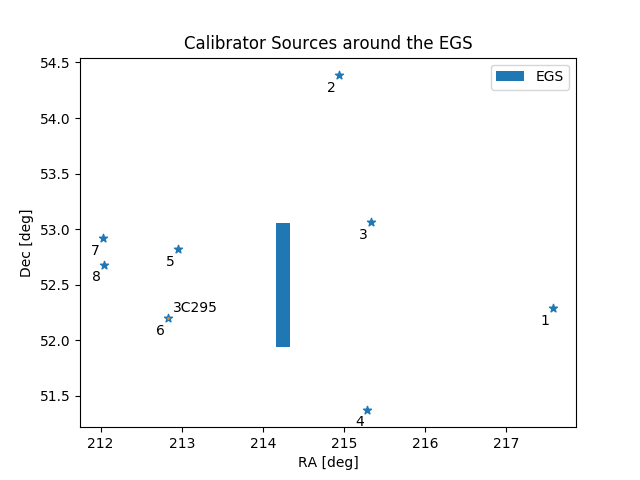
\includegraphics[width=0.8\linewidth]{images/EGS_LOBOS_scatterplot}
%\caption{Position of the calibrator sources around the EGS. Note that this is not projected properly onto the celestial sphere.}
%\label{bootes-coverage-image}
%\end{figure}

\pg
If directional gains are measured to have little or no impact, then direction-dependent calibration of the international stations will not be required. This is the ideal scenario, as it does not require the use of fringe fitting \citepads{1984ARA&A..22...97P}. If they are measured to have a significant impact, then direction-dependent calibration will be required for international LOFAR. We expect the angular scale of differential gain evolution to be of the order of a degree, and so most of the EGS should be relatively unaffected.
%
%\pg
%Having quantified the impact of directional gain errors on our field, we then proceed to a patchwise imaging of the EGS.

%
%
%\subsection{Imaging the EGS with LOFAR international stations}
%
%\pg
%if decorrelation is merciful, proceed to patchwise imaging of EGS by using the results from the sections above (DI calibration using 3c295 model, followed by subtraction of all sources seen at low-res except within the patch we want to image; image, change patch; repeat until all EGS imaged)
%
%\newpage